\chapter{Kiến thức nền tảng}

\section{Học tăng cường (Reinforcement Learning)}

\subsection{Giới thiệu}
Học tăng cường (Reinforcement Learning) \cite{reinforcementlearninganintroduction} là học cách ánh xạ các tình huống thành hành động — để cực đại phần thưởng. Người học không được cho biết hành động nào cần thực hiện, nhưng thay vào đó phải khám phá ra hành động nào mang lại nhiều phần thưởng nhất bằng cách thử chúng. Trong những trường hợp thú vị và khó khăn nhất, các hành động có thể không chỉ ảnh hưởng đến phần thưởng mà còn ảnh hưởng đến tình huống tiếp theo và thông qua đó, cũng ảnh hưởng đến tất cả các phần thưởng tiếp theo. Hai đặc điểm này — tìm kiếm thử-và-sửa sai (trial-and-error) và trì hoãn phần thưởng — là hai đặc điểm phân biệt quan trọng nhất của học tăng cường.

\subsection{Các thành phần của học tăng cường}
Ngoài tác nhân và môi trường, người ta có thể xác định bốn thành phần chính của hệ thống học tăng cường: \textit{policy} (chính sách), \textit{reward signal} (tín hiệu phần thưởng), \textit{value function} (hàm giá trị), và có thể có thêm \textit{model} (mô hình) của \textit{environment} (môi trường).

\begin{itemize}
    \item \textbf{Policy:} xác định cách hoạt động của tác nhân tại một thời điểm nhất định. Nói một cách đại khái, một \textit{policy} là một ánh xạ từ các trạng thái nhận thức của môi trường đến các hành động sẽ được thực hiện khi ở trong các trạng thái đó. Nó tương ứng với những gì trong tâm lý học sẽ được gọi là một tập hợp các quy tắc hoặc liên kết kích thích-phản ứng. Trong một số trường hợp, \textit{policy} có thể là một hàm hoặc bảng tra cứu đơn giản, trong khi trong những trường hợp khác, \textit{policy} có thể liên quan đến tính toán mở rộng chẳng hạn như quá trình tìm kiếm. \textit{Policy} là cốt lõi của một tác nhân học tăng cường theo nghĩa là chỉ nó là đủ để xác định hành vi. Nói chung, các \textit{policy} có thể ngẫu nhiên, chỉ rõ xác suất cho mỗi hành động.
    \item \textbf{Reward signal:} xác định mục tiêu trong vấn đề học tăng cường. Trên mỗi bước thời gian, môi trường gửi cho tác nhân một số duy nhất được gọi là phần thưởng. Mục tiêu duy nhất của tác nhân là tối đa hóa tổng phần thưởng mà tác nhân nhận được trong thời gian dài. Do đó, \textit{reward signal} xác định đâu là những sự kiện tốt và xấu đối với tác nhân. Trong một hệ thống sinh học, chúng ta có thể nghĩ về phần thưởng tương tự như trải nghiệm của niềm vui hoặc nỗi đau. Chúng là các đặc điểm tức thời và xác định vấn đề mà tác nhân phải đối mặt. \textit{Reward signal} là cơ sở chính để thay đổi \textit{policy}; nếu một hành động được \textit{policy} chọn theo sau là \textit{reward} thấp, thì \textit{policy} có thể được thay đổi để chọn một số hành động khác trong tình huống đó trong tương lai. Nói chung, các \textit{reward signal} có thể là các hàm ngẫu nhiên của trạng thái môi trường và các hành động được thực hiện.
    \item \textbf{Value function:} Trong khi \textit{reward signal} cho biết điều gì tốt theo nghĩa tức thời, thì một \textit{value function} chỉ định điều gì tốt về lâu dài. Nói một cách đại khái, \textit{value} của một trạng thái là tổng số phần thưởng mà một tác nhân có thể mong đợi tích lũy trong tương lai, bắt đầu từ trạng thái đó. Trong khi \textit{reward} xác định mong muốn ngay lập tức, nội tại của các trạng thái môi trường, thì các \textit{value} cho thấy mong muốn lâu dài của các trạng thái sau khi tính đến các trạng thái có khả năng tuân theo và \textit{reward} có sẵn trong các trạng thái đó. Ví dụ: một trạng thái có thể luôn mang lại \textit{reward} tức thì thấp nhưng vẫn có \textit{value} cao vì nó thường xuyên được theo sau bởi các trạng thái khác mang lại \textit{reward} cao. Hoặc điều ngược lại có thể đúng. Để so sánh giữa con người với con người, \textit{reward} có phần giống như niềm vui (nếu cao) và nỗi đau (nếu thấp), trong khi \textit{value} tương ứng với sự đánh giá tinh tế hơn và có tầm nhìn xa hơn về mức độ hài lòng hoặc không hài lòng của chúng ta khi môi trường của chúng ta đang ở trong một trạng thái cụ thể.
    \item \textbf{Model environment:} Đây là thứ bắt chước hành vi của môi trường, hay nói chung hơn, cho phép đưa ra các suy luận về cách môi trường sẽ hoạt động. Ví dụ: với một trạng thái và hành động, mô hình có thể dự đoán trạng thái kết quả tiếp theo và phần thưởng tiếp theo. Mô hình được sử dụng để lập kế hoạch, theo đó chúng ta có thể quyết định một quá trình hành động bằng cách xem xét các tình huống có thể xảy ra trong tương lai trước khi chúng thực sự trải qua.
\end{itemize}

\subsection{Ứng dụng của học tăng cường}
Do tính chất của việc học tăng cường là luôn tối ưu việc đạt được phần thưởng cuối cùng dựa vào trạng thái, và phần thưởng hiện tại, cùng với sự tác động của môi trường nên việc học tăng cường được áp dụng nhiều trong các lĩnh vực mang đậm tính tương tác lâu dài giữa \textit{agent} và \textit{environment}, có thể kể đến:

\begin{itemize}
    \item Điều khiển xe tự hành, robot, v.v.
    \item Các hệ thống gợi ý (Recommendation System), hỏi đáp (Chatbot), v.v.
    \item Ngành công nghiệp trò chơi (game) như là cờ vây (nổi tiếng với AlphaGo), v.v.
\end{itemize}

\section{Học tăng cường cho Chatbot hướng mục tiêu (Goal Oriented Chatbot)}

\subsection{Chatbot hướng mục tiêu}
\label{subsec:chatbotgo}
Một Chatbot hướng mục tiêu (GO) \cite{traininggochatbot} cố gắng giải quyết một vấn đề cụ thể cho người dùng. Các Chatbot này có thể giúp mọi người đặt vé, tìm đặt chỗ, v.v. Có hai cách chính để đào tạo một Chatbot GO: Học có giám sát (supervised learning) với bộ mã hóa-giải mã (encoder-decoder), ánh xạ trực tiếp cuộc đối thoại của người dùng tới phản hồi và học tăng cường giúp đào tạo một Chatbot thông qua các cuộc hội thoại thử-và-sửa sai (trial-and-error) với người dùng thực hoặc trình mô phỏng người dùng có quy tắc.

\subsection{Kiến trúc tổng quát của hệ thống Chatbot GO}
Hệ thống đối thoại cho một Chatbot GO sử dụng phương pháp học tăng cường được chia thành 3 phần chính, được mô tả như hình \ref{fig:chatbot}: Phần Quản lý đối thoại (Dialogue Manager), phần Hiểu ngôn ngữ tự nhiên (Natural Language Understanding) và phần Trình tạo ngôn ngữ tự nhiên (Natural Language Generator). Phần Quản lý đối thoại được chia thành Bộ theo dõi trạng thái đối thoại (Dialogue State Tracker) và policy cho chính tác nhân, được đại diện bởi mạng nơ-ron (neural network) trong nhiều trường hợp. Ngoài ra, vòng lặp hệ thống chứa một người dùng với các mục tiêu. Mục tiêu người dùng thể hiện những gì người dùng muốn để thoát khỏi cuộc trò chuyện.

\begin{center}
    \begin{figure}[h!]
        \begin{center}
         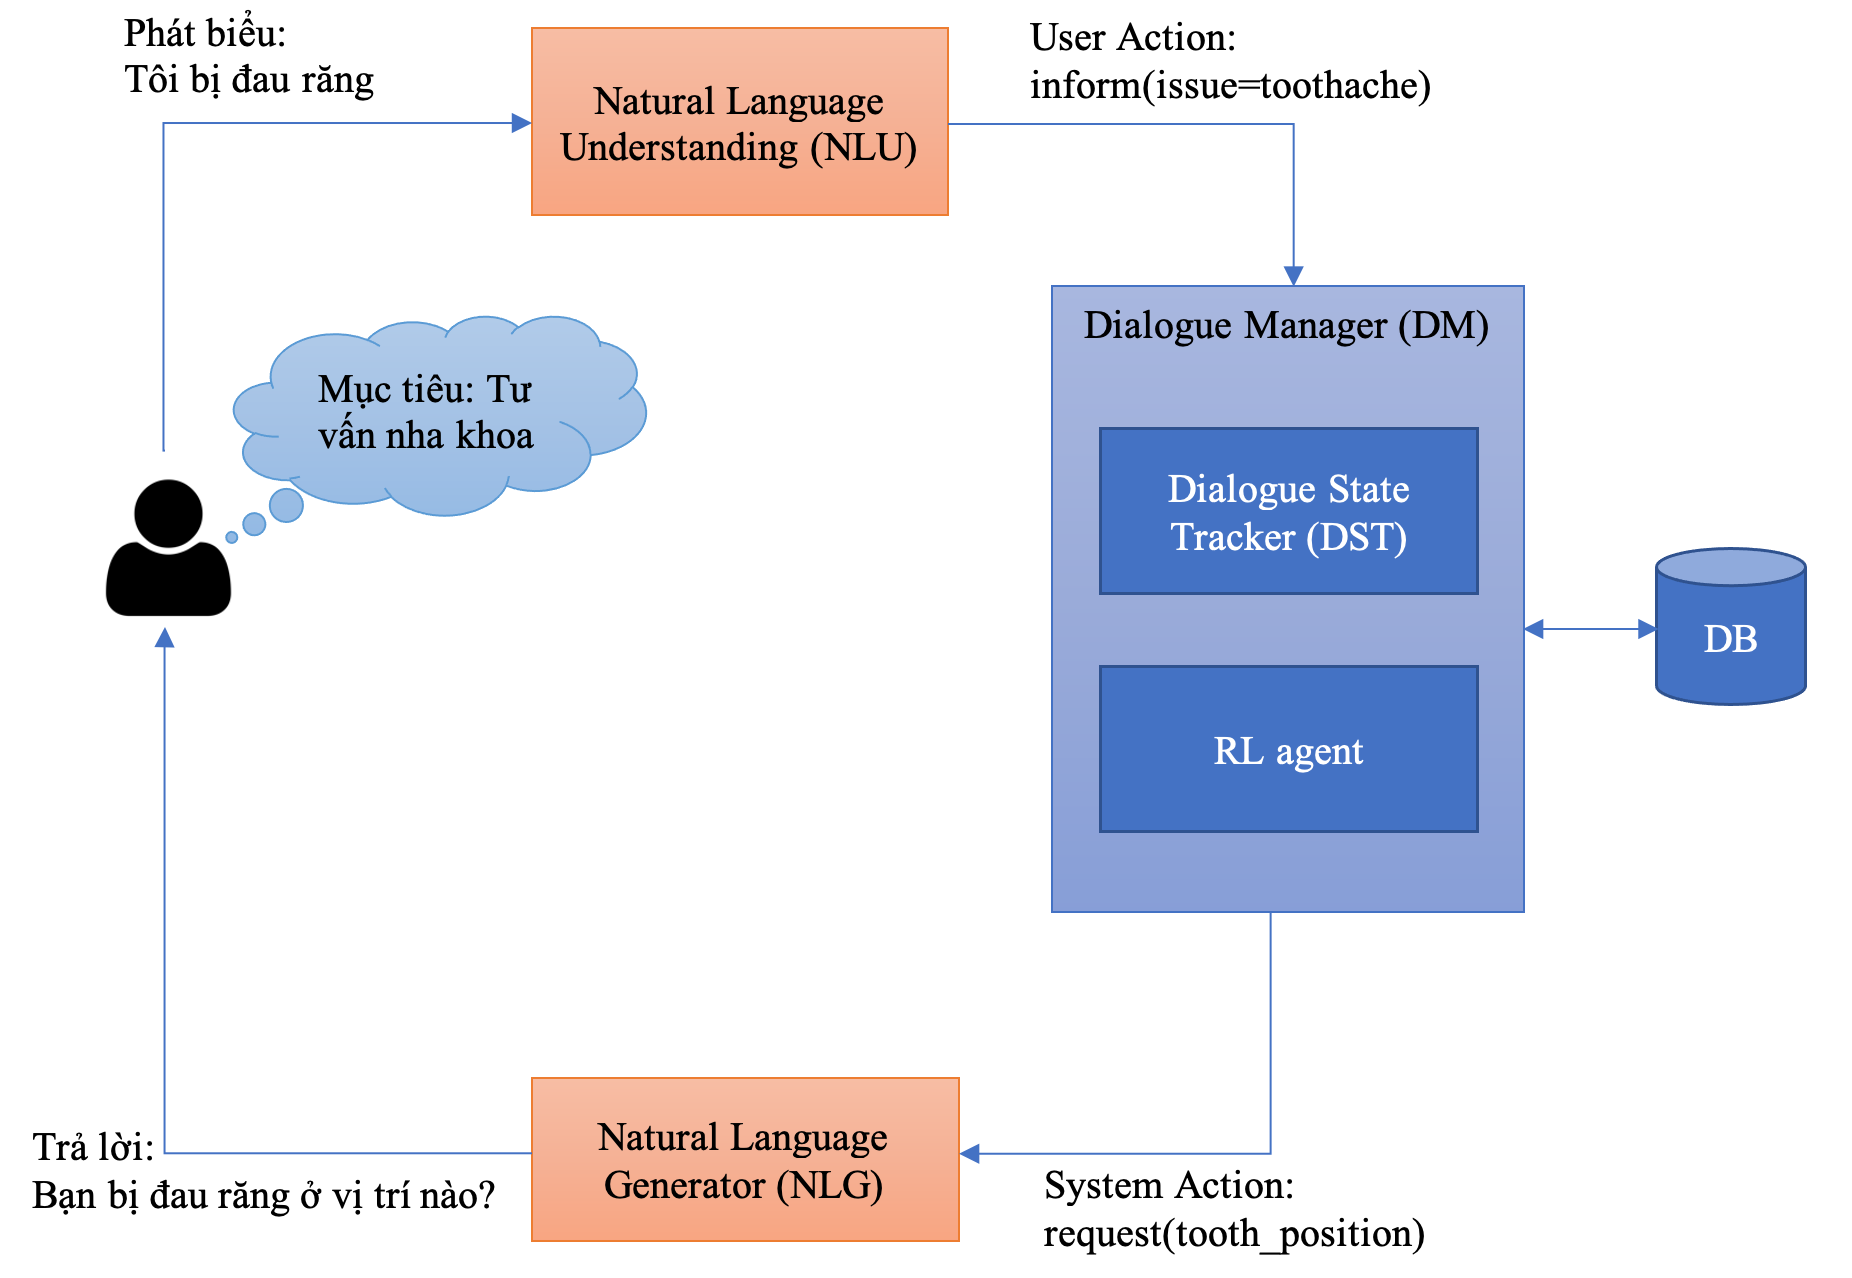
\includegraphics[scale=0.47]{chapter3/img/chatbot.png}
        \end{center}
        \caption{Kiến trúc tổng quát của mô hình Chatbot GO sử dụng phương pháp học tăng cường}
        \label{fig:chatbot}
    \end{figure}
\end{center}

Khi người dùng gửi đi một thông điệp (Tôi bị đau răng), sẽ được xử lý bởi thành phần Hiểu ngôn ngữ tự nhiên (NLU), chuyển ngôn ngữ tự nhiên thành một dạng mà agent có thể xử lý, đầu ra (output) là ở dạng khung ngữ nghĩa (semantic frame) (inform(issue=toothache)).

Sau đó, Bộ theo dõi trạng thái đối thoại (DST) từ hành động của người dùng (đã được chuyển thành khung ngữ nghĩa) và lịch sử của cuộc trò chuyện hiện tại sẽ xử lý và chuyển thành một biểu diễn trạng thái mà có thể xử lý được bởi policy của agent. Trạng thái này là đầu vào của policy hoặc mạng nơ ron của agent, output là hành động của agent dưới dạng khung ngữ nghĩa. (request(tooth\_position))

Cơ sở dữ liệu được truy vấn để thêm thông tin vào cho agent như thông tin các loại bệnh và triệu chứng, v.v.

Hành động của agent sau đó được xử lý bởi phần Trình tạo ngôn ngữ tự nhiên (NLG), chuyển nó sang ngôn ngữ tự nhiên để người dùng có thể dễ dàng đọc hiểu (Bạn bị đau răng ở vị trí nào?).

\section{Mô hình học tăng cường cho Chatbot GO}
\label{sec:model}
Như đã đề cập ở mục \ref{subsec:chatbotgo}, mục đích của tác nhân (agent) Chatbot hướng mục tiêu (GO) là được đào tạo để trò chuyện thành thạo với người dùng thực nhằm hoàn thành mục tiêu, phù hợp với các ràng buộc của người dùng. Công việc chính của \textit{agent} là đưa ra trạng thái và tạo ra một hành động gần đến mức tối ưu. Cụ thể, \textit{agent} nhận được một trạng thái đại diện cho lịch sử của cuộc trò chuyện hiện tại từ Bộ theo dõi trạng thái đối thoại (DST) và chọn một phản hồi trả về cho cuộc đối thoại. Để giải quyết cho bài toán trên, ta sử dụng mô hình Deep Q-Learning.

\subsection{Q-Learning}
Giả sử, \textit{agent} đang ở trạng thái $s$ và phải chọn một hành động $a$, nó sẽ nhận được phần thưởng $r$ và đạt trạng thái mới $s'$. Cách mà \textit{agent} chọn được gọi là \textit{policy}.

\begin{equation*}
    s \xrightarrow{\text{a}} r,s'
\end{equation*}

Ta định nghĩa một hàm $Q(s,a)$ sao cho khi nhận vào trạng thái $s$ và hành động $a$ nó sẽ trả về một giá trị ước lượng là tổng phần thưởng mà ta sẽ đạt được tại trạng thái đó khi ta thực hiện hành động $a$ và thực hiện một số \textit{policy} tiếp theo sau đó. Ta chắc chắn rằng sẽ luôn có các \textit{policy} tối ưu, nghĩa là nó luôn chọn được hành động tốt nhất. Ta gọi hàm $Q$ trong trường hợp luôn có \textit{policy} tối ưu là $Q^*$. Nếu ta biết được hàm $Q^*$, ta chỉ cần áp dụng chiến lược tham lam (greedy) lên hàm đó. Cụ thể với mỗi trạng thái $s$, ta sẽ chọn một hành động $a$ sao cho cực đại hoá hàm $Q^*$, hay ${argmax_a}{Q^*}(s,a)$. Mục tiêu của chúng ta là tìm được hàm đủ tốt để ước lượng được hàm $Q^*$ rồi sau đó áp dụng chiến lược tham lam lên nó. Ta viết lại hàm $Q^*$ ở dạng sau:

\begin{equation*}
    Q^*(s,a) = r_0 + {\gamma}r_1 + {\gamma}^{2}r_2 + {\gamma}^{3}r_3 + ...
\end{equation*}

Hàm $Q^*$ lúc này là tổng giá trị của phần thưởng nhận được sau mỗi hành động tính từ hành động $a$ trở đi. $\gamma$ là giá trị khấu hao của phần thưởng sau mỗi hành động và nó luôn nhỏ hơn 1 để đảm bảo rằng công thức này có giới hạn. Vì có hệ số mũ nên giá trị phần thưởng sẽ giảm dần và tiến về 0. Hệ số $\gamma$ vì vậy mà sẽ điều khiển mức độ phụ thuộc vào tương lai của hàm $Q$ tại trạng thái $s$.\newline

Ta có thể viết lại hàm $Q^*$ ở trên như sau:

\begin{equation*}
    Q^*(s,a) = r_0 + {\gamma}(r_1 + {\gamma}r_2 + {\gamma}^{2}r_3 + ...) = r_0 + {\gamma}argmax_{a}Q^{*}(s',a)
\end{equation*}

Công thức này cho thấy giá trị hàm $Q$ của hành động $a$ tại trạng thái $s$ bằng phần thưởng $r(s,a)$ cộng với giá trị hàm $Q$ lớn nhất của các trạng thái $s'$ tiếp theo khi thực hiện các hành động $a$. Do đó, với công thức này chúng ta có thể tạo ra một ma trận trạng thái-hành động (state-action) như một bảng tìm kiếm (lookup table). Từ đó với mỗi trạng thái, \textit{agent} chỉ cần tìm hành động nào có giá trị hàm $Q$ lớn nhất là xong.\newline

Tuy nhiên, trong thực tế số lượng trạng thái rất lớn và ta không thể nào lưu trữ toàn bộ chúng như cách ở trên được. Vì vậy ta sẽ xấp xỉ hàm $Q$ bằng một mạng nơ-ron. Mạng nơ-ron này sẽ nhận đầu vào là một trạng thái và nó sẽ ước lượng giá trị của hàm $Q$ cho mỗi một hành động. Và khi ta sử dụng nhiều tầng, ta được mạng nơ-ron học sâu.

\subsection{Deep Q-Learning}
Q-Learning hoạt động tốt khi chúng ta có một môi trường tương đối đơn giản để giải quyết, nhưng khi số lượng trạng thái và hành động chúng ta có thể thực hiện trở nên phức tạp hơn, chúng ta sử dụng deep learning như một công cụ xấp xỉ hàm.

Trạng thái được đưa ra làm đầu vào và giá trị Q của tất cả các hành động có thể được tạo ra làm đầu ra. Sự so sánh giữa Q-learning và Deep Q-Learning được minh họa như hình \ref{fig:dqlearning} \cite{introductiondeepqlearningpython} dưới đây:

\begin{center}
    \begin{figure}[h!]
        \begin{center}
         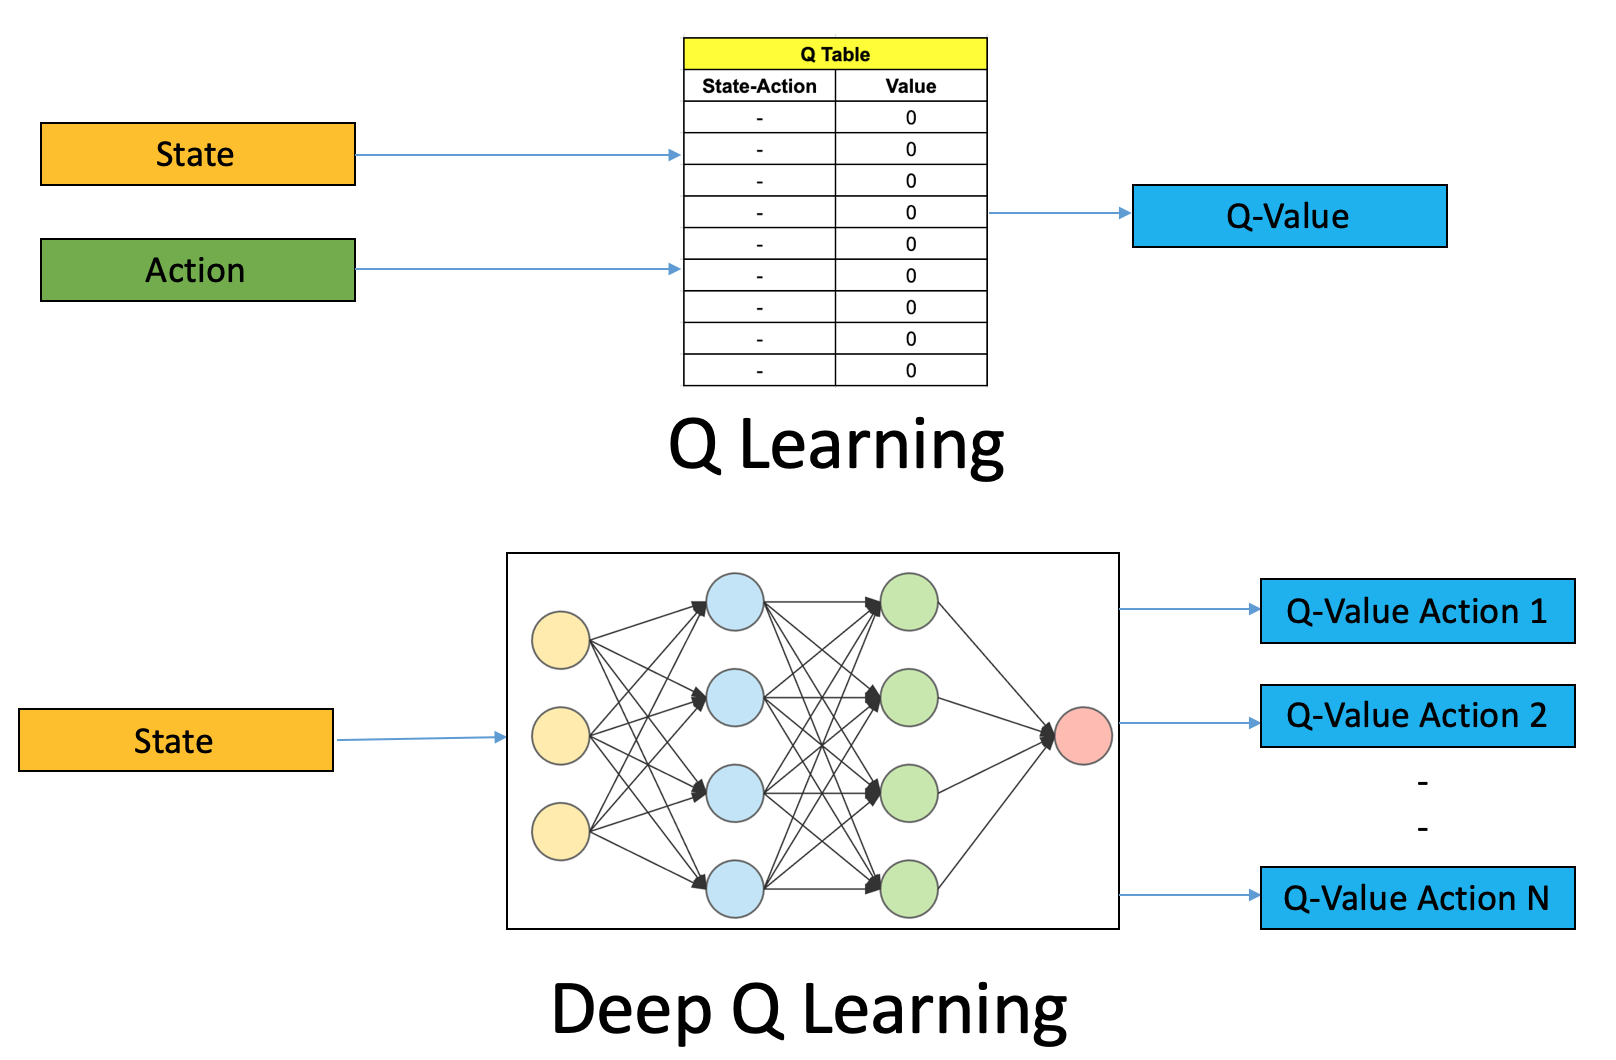
\includegraphics[scale=0.27]{chapter3/img/dqlearning.png}
        \end{center}
        \caption{Q-Learning và Deep Q-Learning}
        \label{fig:dqlearning}
    \end{figure}
\end{center}

